\section{Exploratory Data Analysis}

An effective way to understand and explore a dataset is through visualization of the feature distribution for each class.
However, when the number of features is high, such as 728 in this case, this method may not be practical or informative.
In these situations, alternative approaches for visualizing the dataset can be utilized to extract useful insights.

\subsection{Principal Component Analysis}
One way to gain insights from a large dataset that might be difficult to visualize otherwise is through the use of principal component analysis (PCA).
PCA is a technique that reduces the number of features in a dataset while preserving the most important information.
It does so by transforming the original variables into a new set of variables called principal components, which are uncorrelated and capture the maximum amount of variance in the data.
In the following analysis, we will investigate the relationships between the first three principal components.

\begin{figure}[H]
    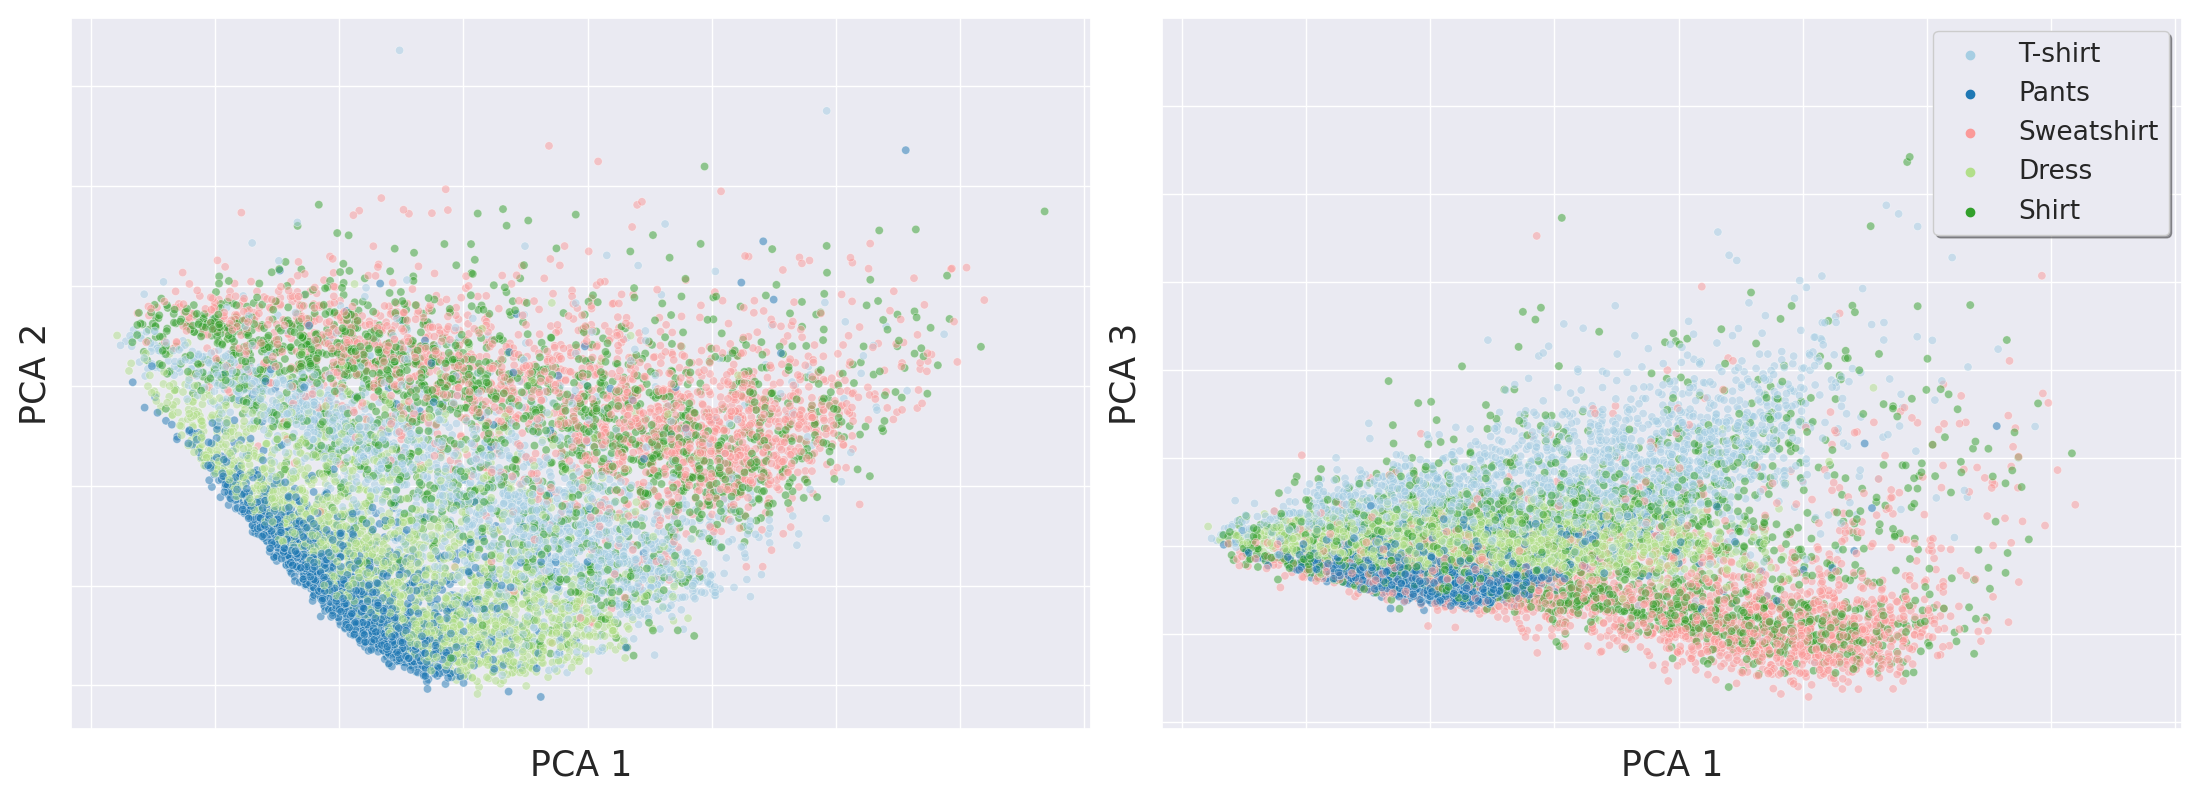
\includegraphics[scale=0.30]{figures_for_report/PCA}
    \captionsetup{justification=centering,margin=2cm}
    \caption{Visualizing relationships between the first 3 principal components}
\end{figure}

The first 3 principal components explain $42.7\%$ variance, and it requires 61 principal components to explain above $90\%$ variance.
PCA plots can be useful for understanding how well the different classes are separated and can provide insight into the difficulty of accurately predicting the various clothing types.
\textbf{Figure 3} demonstrates that there is significant overlap between many of the classes, particularly between Shirts and Pullovers.
This overlap could potentially make it difficult for a classifier to distinguish between these two classes.
For dresses and trousers the opposite seems to be the case - their PCA plot profile is much more distinct.
In section \textbf{4}, \textbf{5} and \textbf{6} below three different methods for determining the type of clothing from an
image is explored.
